\documentclass[11pt]{article}
\usepackage{deauthor,graphicx,times}
\usepackage{cite}

% COMMANDS GO HERE
%please list all commands used in your paper, eliminating duplicates

\newtheorem{Example}{\textbf{Example}}


% Your paper submission must be in a folder named with the
% contact author name.

\graphicspath{{author-name/}}

\begin{document}


%\title{Data Errors: Symptoms, Causes and Origins}

%% \author{
%% Ihab F. Ilyas \\
%% University of Waterloo\\ Canada  \\
%%  ilyas@cs.uwaterloo.ca\\
%% \and Felix Naumann\\
%%  Hasso Plattner Institute, University of Potsdam\\Germany \\
%%  felix.naumann@hpi.de
%% }

%% \maketitle

%\begin{abstract}
%\end{abstract}

%%!TEX root = paper.tex
\section{Introduction: Data Errors and their Root Causes}
\label{sec:intro}

With the recent move towards data-centric AI, data quality is now playing an even bigger role in producing sound and reliable insights, predictions and analytics. While the data management community has been working on the problem of data cleaning for decades, the problem remains very much present. Most efforts have focused on error detection~\cite{DBLP:books/acm/IlyasC19}, attempting to leverage symptoms and the manifestations of these errors in data sets to locate and possibly repair them. 
Indeed, the last few years witnessed significant advances in automating error detection and repairing~\cite{holoclean,holodetect,raha,yeye-unidetect} by probabilistically modelling dirty data sets, and reasoning about error detection and repair as structured prediction problems~\cite{puds,uai_heidari}. In this opinion piece, we present our views on how to further advance the field of data cleaning, and go beyond treating the symptoms of the problem and understand what it takes to treat the causes and the sources of these anomalies and errors.

Tracking errors to their sources is not a new quest of the research community~\cite{DBLP:conf/sigmod/ChalamallaIOP14, DBLP:conf/sigmod/WangM017, DBLP:journals/ftdb/GlavicMR21}. So why are we revisiting it now? %The main observation that motivates this discussion is 
The way current research currently reasons about the root causes of data errors is still, in our opinion, limited. \emph{Tracking errors to sources} has often been framed as  ``computational'' provenance that represents \emph{what} was involved in computing a final data product and possibly \emph{how} this product was computed. The main goal of these provenance-based error tracking systems is projecting errors detected in downstream applications all the way to upstream data sources, where they should be fixed~\cite{DBLP:conf/sigmod/ChalamallaIOP14}.  While the principle is sound, multiple issues often complicate this approach. First, as data processing pipelines become more complex, with cascades of complex machine learning models, capturing this rich provenance information becomes harder, as most if not all of the input is involved in producing the output. Recent progress, however, has been made in tracking responsibility of training data, for example, in the predictions of complex models~\cite{DBLP:journals/corr/abs-2002-08484,pmlr-koh-Liang,DBLP:journals/corr/abs-2202-00622}. Second, even with advances in modelling the responsibility of input sources in the observations in output analytics reports, fixing the sources does not mean that errors have been fixed at their true ``roots'' -- their point of creation; these raw data sources are often the results of other processes not modelled at all in the computational data pipelines, such as grading tasks of humans, sensor readings, and extraction scripts from logs and documents.  

Hence, we argue that effective management of data errors and the next-generation data cleaning systems require a more profound understanding of the root causes data errors. These systems should: (1)~distinguish between \emph{why} errors occur and the processes that generated them in the first place, and \emph{how}  these errors manifest themselves as bad data symptoms (e.g., violations of integrity constraints and appearing as outlying values), and (2)~explicitly model these data generation processes to allow for new process repair actions that go beyond fixing raw data sources. 

% NEED TO INTEGRATE THE FOLLOWING SOMEHOW 
%
%In the absence of any context, a data element\footnote{For now, we formulate our definitions in the most general way by referring to ``data elements'', which can manifest as individual values, rows, columns, objects, graphs, tables or entire datasets. Later, we supply details on this ``what'' question.} cannot constitute an error -- it just ``is''. However, data elements do not exist outside some context: they were somehow produced and shall somehow be consumed. Only this context allows us to identify a data element as erroneous. We can ask \emph{how} the element is an error: how do we notice it as erroneous, what symptoms does it hold? These symptoms exist only in the context of the consumption of the data element. For instance, data might violate some external constraint or assumption. It might be an outlier, compared to other data elements. A relation might be missing some tuples or have some duplicated tuples.

%Given such identified errors, we can ask the obvious next question: \emph{Why} do we observe the error, how did it appear in the data? Possible answers to these questions are the provenance of the data, and the mode in which the data was originally created. For instance, human data entry can create such errors, or faulty sensors produce erroneous data.



%!TEX root = paper.tex
\section{Introduction: Data Errors and their Root Causes}
\label{sec:intro}

With the recent move towards data-centric AI, data quality is now playing an even bigger role in producing sound and reliable insights, predictions and analytics. While the data management community has been working on the problem of data cleaning for decades, the problem remains very much present. Most efforts have focused on error detection~\cite{DBLP:books/acm/IlyasC19}, attempting to leverage symptoms and the manifestations of these errors in data sets to locate and possibly repair them. 
Indeed, the last few years witnessed significant advances in automating error detection and repairing~\cite{holoclean,holodetect,raha,yeye-unidetect} by probabilistically modelling dirty data sets, and reasoning about error detection and repair as structured prediction problems~\cite{puds,uai_heidari}. In this opinion piece, we present our views on how to further advance the field of data cleaning, and go beyond treating the symptoms of the problem and understand what it takes to treat the causes and the sources of these anomalies and errors.

Tracking errors to their sources is not a new quest of the research community~\cite{DBLP:conf/sigmod/ChalamallaIOP14, DBLP:conf/sigmod/WangM017, DBLP:journals/ftdb/GlavicMR21}. So why are we revisiting it now? %The main observation that motivates this discussion is 
The way current research currently reasons about the root causes of data errors is still, in our opinion, limited. \emph{Tracking errors to sources} has often been framed as  ``computational'' provenance that represents \emph{what} was involved in computing a final data product and possibly \emph{how} this product was computed. The main goal of these provenance-based error tracking systems is projecting errors detected in downstream applications all the way to upstream data sources, where they should be fixed~\cite{DBLP:conf/sigmod/ChalamallaIOP14}.  While the principle is sound, multiple issues often complicate this approach. First, as data processing pipelines become more complex, with cascades of complex machine learning models, capturing this rich provenance information becomes harder, as most if not all of the input is involved in producing the output. Recent progress, however, has been made in tracking responsibility of training data, for example, in the predictions of complex models~\cite{DBLP:journals/corr/abs-2002-08484,pmlr-koh-Liang,DBLP:journals/corr/abs-2202-00622}. Second, even with advances in modelling the responsibility of input sources in the observations in output analytics reports, fixing the sources does not mean that errors have been fixed at their true ``roots'' -- their point of creation; these raw data sources are often the results of other processes not modelled at all in the computational data pipelines, such as grading tasks of humans, sensor readings, and extraction scripts from logs and documents.  

Hence, we argue that effective management of data errors and the next-generation data cleaning systems require a more profound understanding of the root causes data errors. These systems should: (1)~distinguish between \emph{why} errors occur and the processes that generated them in the first place, and \emph{how}  these errors manifest themselves as bad data symptoms (e.g., violations of integrity constraints and appearing as outlying values), and (2)~explicitly model these data generation processes to allow for new process repair actions that go beyond fixing raw data sources. 

% NEED TO INTEGRATE THE FOLLOWING SOMEHOW 
%
%In the absence of any context, a data element\footnote{For now, we formulate our definitions in the most general way by referring to ``data elements'', which can manifest as individual values, rows, columns, objects, graphs, tables or entire datasets. Later, we supply details on this ``what'' question.} cannot constitute an error -- it just ``is''. However, data elements do not exist outside some context: they were somehow produced and shall somehow be consumed. Only this context allows us to identify a data element as erroneous. We can ask \emph{how} the element is an error: how do we notice it as erroneous, what symptoms does it hold? These symptoms exist only in the context of the consumption of the data element. For instance, data might violate some external constraint or assumption. It might be an outlier, compared to other data elements. A relation might be missing some tuples or have some duplicated tuples.

%Given such identified errors, we can ask the obvious next question: \emph{Why} do we observe the error, how did it appear in the data? Possible answers to these questions are the provenance of the data, and the mode in which the data was originally created. For instance, human data entry can create such errors, or faulty sensors produce erroneous data.


%%!TEX root = paper.tex
\section{Reasoning about the How: The Symptoms of Errors}
\label{sec:how}

In its most general form, information quality is defined as ``fitness for use''~\cite{Strong96}, i.e., its definition focuses on the use case, the application, the \emph{context} of the data at hand. Most, if not all, error detection methods make heavy use of this context. They search for and focus on the \emph{symptoms} of poor data quality and ask the question \emph{how} a particular data element is an error.
We exemplify this insight with selected examples of traditional error detection problems and their solutions.
\begin{description}
  \item[Outliers] Already by definition, outliers can be recognized only in the context of other data elements -- only these ``inliers'' make some other value an outlier. Typical outlier detection methods create a model to represent normal/typical values and mark as outliers all those values that do not fit the model~\cite{Aggarwal2013}. Whether an outlier is, in fact, an error is application-dependent and user-defined.
  
  \emph{How} is an outlier a data error? It is very different from all \emph{other} data elements, suggesting it is not the intended value for this data item.
  
  \item[Constraint violations] Constraints, such as key-constraints, dependencies, or denial constraints can be used to express the validity of a data instance. These rules are specified by experts or discovered with data profiling methods~\cite{Abedjan2018}. Rarely do they refer to individual data elements; rather they forbid the existence of some elements in the presence of others, such as a key-constraint denying any other record with the same key value. Discovering and cleaning such violations is an active research area~\cite{IlyasC15}.
  
  \emph{How} does a data element violate a constraint? It exists in the presence of some \emph{other} data element. While this is not an error on its own, the collection of these values cannot be part of the intended correct data instance. %, together with which it violates the constraint.
  
  \item[Duplicates] Within a dataset, duplicate records are multiple different representations of the same real-world entity~\cite{Naumann10}. To clean a dataset, such erroneous duplicates must be detected and then merged or eliminated. Identifying a duplicated record is, by definition, possible only by regarding other records, i.e., only in the context of the entire relation. Typical approaches intelligently create duplicate candidate pairs and then determine their similarity to decide whether they are indeed duplicates~\cite{Papadakis21}.
  
  \emph{How} is a duplicate an error? It represents the same real-world object as some \emph{other} data element, with possibly other types of errors causing a different representation.
  
  \item[Missing values] Missing values are easy to detect when they appear as null values in databases or empty strings in files. In more complex cases, ``disguised missing values'' can be recognized only by regarding their context, which usually comprises the other values in the column~\cite{FAHES_18}. 
  The typical means to ``clean'' missing values is to impute their value, again based on their context, usually the non-missing values in a column.
  
  \emph{How} is a missing value an error? It is explicitly represented to indicate an error. However, the difficulty in the case of missing value relates to the interpretation of ``null'' as {\em we don't know the value, but we should} as opposed to schema issues, for example, a relational employees table with some employees who do not have middle names.
\end{description}

Data cleaning, as a means to alleviate the symptoms of poor data quality, is an established and important research and development field, relying heavily on the context of data and its use in applications. Next, we move backwards along the data processing pipeline to explore not these symptoms, but their causes.
%!TEX root = paper.tex
\section{Reasoning about the How: The Symptoms of Errors}
\label{sec:how}

In its most general form, information quality is defined as ``fitness for use''~\cite{Strong96}, i.e., its definition focuses on the use case, the application, the \emph{context} of the data at hand. Most, if not all, error detection methods make heavy use of this context. They search for and focus on the \emph{symptoms} of poor data quality and ask the question \emph{how} a particular data element is an error.
We exemplify this insight with selected examples of traditional error detection problems and their solutions.
\begin{description}
  \item[Outliers] Already by definition, outliers can be recognized only in the context of other data elements -- only these ``inliers'' make some other value an outlier. Typical outlier detection methods create a model to represent normal/typical values and mark as outliers all those values that do not fit the model~\cite{Aggarwal2013}. Whether an outlier is, in fact, an error is application-dependent and user-defined.
  
  \emph{How} is an outlier a data error? It is very different from all \emph{other} data elements, suggesting it is not the intended value for this data item.
  
  \item[Constraint violations] Constraints, such as key-constraints, dependencies, or denial constraints can be used to express the validity of a data instance. These rules are specified by experts or discovered with data profiling methods~\cite{Abedjan2018}. Rarely do they refer to individual data elements; rather they forbid the existence of some elements in the presence of others, such as a key-constraint denying any other record with the same key value. Discovering and cleaning such violations is an active research area~\cite{IlyasC15}.
  
  \emph{How} does a data element violate a constraint? It exists in the presence of some \emph{other} data element. While this is not an error on its own, the collection of these values cannot be part of the intended correct data instance. %, together with which it violates the constraint.
  
  \item[Duplicates] Within a dataset, duplicate records are multiple different representations of the same real-world entity~\cite{Naumann10}. To clean a dataset, such erroneous duplicates must be detected and then merged or eliminated. Identifying a duplicated record is, by definition, possible only by regarding other records, i.e., only in the context of the entire relation. Typical approaches intelligently create duplicate candidate pairs and then determine their similarity to decide whether they are indeed duplicates~\cite{Papadakis21}.
  
  \emph{How} is a duplicate an error? It represents the same real-world object as some \emph{other} data element, with possibly other types of errors causing a different representation.
  
  \item[Missing values] Missing values are easy to detect when they appear as null values in databases or empty strings in files. In more complex cases, ``disguised missing values'' can be recognized only by regarding their context, which usually comprises the other values in the column~\cite{FAHES_18}. 
  The typical means to ``clean'' missing values is to impute their value, again based on their context, usually the non-missing values in a column.
  
  \emph{How} is a missing value an error? It is explicitly represented to indicate an error. However, the difficulty in the case of missing value relates to the interpretation of ``null'' as {\em we don't know the value, but we should} as opposed to schema issues, for example, a relational employees table with some employees who do not have middle names.
\end{description}

Data cleaning, as a means to alleviate the symptoms of poor data quality, is an established and important research and development field, relying heavily on the context of data and its use in applications. Next, we move backwards along the data processing pipeline to explore not these symptoms, but their causes.

%%!TEX root = paper.tex
\section{Reasoning about the Why: The Causes of Errors}
\label{sec:why}

It is time to ask (and answer) the \emph{why} question!
Existing work in the area of data quality, error detection and data cleaning almost exclusively focuses on alleviating the symptoms, rather than removing the cause of the error.
None of the methods asks \emph{why} a particular value is missing, why duplicates exist in the data, why violations occur. Answers as to ``why'' include: faulty (human) data entry, such as missing entries, misplaced values, typos, and vandalism; faulty reading from sensors; missed or not-propagated updates; faulty computations; and misconfigured data pipelines. 

While researchers and practitioners (and medical doctors) will acknowledge the truism that problems are best addressed at their source rather than treating their symptoms, the research community has not adequately addressed this opportunity possibly for several reasons:
\begin{itemize}
    \item In some scenarios, once errors are detected, it is too late -- fixing their cause is futile because the data was intended for a one-time use.
    \item Often, the creation of data is out of the control of the data engineers or data consumers: the data stems from an external source and the data creation can be influenced only through human intervention, such as communicating with the data owners or creators.
    \item Modifying or improving the data creation process is difficult or impossible, for instance due to technical or human limitations: sensors have an inherent error margin; humans are not infallible, etc.
    \item Data processing pipelines have become so complex, that treating the symptoms is the easier short-term goal with quick rewards.
\end{itemize}

Knowledge of the cause of an error and not only its symptom can improve cleaning methods and can help avoid such errors in the first place. To seize this opportunity, multiple challenges must be overcome:
\begin{itemize}
    \item \emph{Modelling} the processes and data generators (including humans) in the system, instead of modelling only the data and errors.

    \item \emph{Detection} of data errors without context and detection of erroneous data processes.
    
    \item Extending the notion of \emph{provenance} to include (possibly faulty) processes, computation (internal provenance), and data generation steps (external provenance). More on this in Section\ref{sec:provenance}.
    
    \item Designing of algorithms and systems to efficiently and effectively trace such extended provenance.
    
    \item Designing \emph{repair} operations for such errors and processes, which need to reach beyond the mere deletion or replacement of data instances that is the currently common approach.

%    \item Algorithms that can point to these new things
\end{itemize}

These challenges can be summarized as creating a more holistic view of data creation and consumption than is currently practiced. Especially the extended notion of provenance deserves a closer look in the next section.

%existing work: Modelling the process or Cleaning actions at the source

%Definition of cause of error: SOME TEXT. Understanding the cause of an error asks ``Why do we observe this error?''

%Raw-data generative process (link to ICDT paper by Ihab, and others)


%``So I'll remove the cause. But not. The symptom!'' Dr.\ Frank N.\ Furter, Rocky Horror Picture Show
%!TEX root = paper.tex
\section{Reasoning about the Why: The Causes of Errors}
\label{sec:why}

It is time to ask (and answer) the \emph{why} question!
Existing work in the area of data quality, error detection and data cleaning almost exclusively focuses on alleviating the symptoms, rather than removing the cause of the error.
None of the methods asks \emph{why} a particular value is missing, why duplicates exist in the data, why violations occur. Answers as to ``why'' include: faulty (human) data entry, such as missing entries, misplaced values, typos, and vandalism; faulty reading from sensors; missed or not-propagated updates; faulty computations; and misconfigured data pipelines. 

While researchers and practitioners (and medical doctors) will acknowledge the truism that problems are best addressed at their source rather than treating their symptoms, the research community has not adequately addressed this opportunity possibly for several reasons:
\begin{itemize}
    \item In some scenarios, once errors are detected, it is too late -- fixing their cause is futile because the data was intended for a one-time use.
    \item Often, the creation of data is out of the control of the data engineers or data consumers: the data stems from an external source and the data creation can be influenced only through human intervention, such as communicating with the data owners or creators.
    \item Modifying or improving the data creation process is difficult or impossible, for instance due to technical or human limitations: sensors have an inherent error margin; humans are not infallible, etc.
    \item Data processing pipelines have become so complex, that treating the symptoms is the easier short-term goal with quick rewards.
\end{itemize}

Knowledge of the cause of an error and not only its symptom can improve cleaning methods and can help avoid such errors in the first place. To seize this opportunity, multiple challenges must be overcome:
\begin{itemize}
    \item \emph{Modelling} the processes and data generators (including humans) in the system, instead of modelling only the data and errors.

    \item \emph{Detection} of data errors without context and detection of erroneous data processes.
    
    \item Extending the notion of \emph{provenance} to include (possibly faulty) processes, computation (internal provenance), and data generation steps (external provenance). More on this in Section\ref{sec:provenance}.
    
    \item Designing of algorithms and systems to efficiently and effectively trace such extended provenance.
    
    \item Designing \emph{repair} operations for such errors and processes, which need to reach beyond the mere deletion or replacement of data instances that is the currently common approach.

%    \item Algorithms that can point to these new things
\end{itemize}

These challenges can be summarized as creating a more holistic view of data creation and consumption than is currently practiced. Especially the extended notion of provenance deserves a closer look in the next section.

%existing work: Modelling the process or Cleaning actions at the source

%Definition of cause of error: SOME TEXT. Understanding the cause of an error asks ``Why do we observe this error?''

%Raw-data generative process (link to ICDT paper by Ihab, and others)


%``So I'll remove the cause. But not. The symptom!'' Dr.\ Frank N.\ Furter, Rocky Horror Picture Show
%%!TEX root = paper.tex
\section{True Data Provenance}
\label{sec:provenance}

Provenance is powerful tool for {\em tracking} data artifacts. In the context of this paper, one might think of it as a way to identify the \emph{where} of the data error's story. Most practical and effective cleaning solutions follow a clean-and-evaluate lifecycle~\cite{Ilyas16DE}, which leverages the computational provenance of data analytics to track data errors to their sources, and attempts to provide explanations that lead to cleaning actions. This typical lifecycle is depicted in Figure~\ref{fig:lifecycle}. 
\begin{figure*}[ht]
  \centering
  \includegraphics[width=0.6\textwidth]{lifecycle}
  \caption{Clean-and-Evaluate Loop~\cite{Ilyas16DE}}
  \label{fig:lifecycle}
\end{figure*}

Provenance and lineage systems focus on describing how the analytical {\em report views} are computed from the sources. For example, Scorpion~\cite{DBLP:journals/pvldb/0002M13}, DBRx~\cite{DBLP:conf/sigmod/ChalamallaIOP14} and QFix~\cite{DBLP:conf/sigmod/WangM017} (and many other followup work) are  solutions that trace back the tuples that contributed to the problems in the target to explain and help fix these errors at data sources. A recent survey summarizes the large body of work in debugging data-driven systems and explain what users see downstream from processing raw data~\cite{DBLP:journals/ftdb/GlavicMR21}. As these processing pipelines become more complex with cascades of large machine learning models, tracing errors in final predictions back to their causes can be very challenging. However, there is recent progress that can help us reason about observations in model predictions and track them back to errors in training data~\cite{DBLP:journals/corr/abs-2202-00622}.

The question becomes: \emph{is explaining errors in final analytics or predictions in terms of data sources enough?} What we refer to as ``raw data sources''  are often cut off the processes that generated these data, such as the human grader that input that data, the extraction script that generated this data from a webpage, or a presentation of the complex data pipeline that ran in a different software stack and generated this source data. From our discussions and involvement with large enterprises over the last decade, we argue that this decoupling is often due to two main reasons:
\begin{itemize}
\item \emph{Difficulty of integrating data processes in provenance systems:} Representing the process that generated the data might require expressive (and hence  complex) provenance systems. For example semiring-based  provenance systems have been extended  to capture information about external inputs (e.g., user choices), and  to capture process executions~\cite{DBLP:journals/vldb/DeutchMT15}; and in the context of scientific workflows,  the need for a control-flow driven workflow provenance model in contrast to the traditional  data-driven execution provenance paradigm has been explored~\cite{DBLP:journals/dke/ButtF21}.

\item \emph{Loss of provenance continuity across systems:}  We might be very careful in collecting and adequately presenting provenance information in the data pipelines we control. However, as the final data product (e.g., predictions, views, aggregates, or transformed data sets) get pushed to the downstream tasks, they are often treated as ``source data'' and downstream pipelines fail to  consume the associated provenance information.
\end{itemize}

Understandably, these are hard problems to tackle and part of the challenge is not even technical and it involves standardizing data provenance representation across business units and different software stacks. However, this might suggest new research directions; for example, we might prefer developing simpler and less expressive provenance models that target interoperability and ease of propagation over representation power of the underlying computations. Another example is that propagating standard meta-data that ties data sources to central data governance and catalogs can be part of the integrity constraints and sanity checks. We suggest also extending meta-data representation of data sources to include {\em repair actions} that reference a controlled vocabulary or a {\em repairing ontology} tapping into the large body of work in work flow and business processes management.





%!TEX root = paper.tex
\section{True Data Provenance}
\label{sec:provenance}

Provenance is powerful tool for {\em tracking} data artifacts. In the context of this paper, one might think of it as a way to identify the \emph{where} of the data error's story. Most practical and effective cleaning solutions follow a clean-and-evaluate lifecycle~\cite{Ilyas16DE}, which leverages the computational provenance of data analytics to track data errors to their sources, and attempts to provide explanations that lead to cleaning actions. This typical lifecycle is depicted in Figure~\ref{fig:lifecycle}. 
\begin{figure*}[ht]
  \centering
  \includegraphics[width=0.6\textwidth]{letters/lifecycle}
  \caption{Clean-and-Evaluate Loop~\cite{Ilyas16DE}}
  \label{fig:lifecycle}
\end{figure*}

Provenance and lineage systems focus on describing how the analytical {\em report views} are computed from the sources. For example, Scorpion~\cite{DBLP:journals/pvldb/0002M13}, DBRx~\cite{DBLP:conf/sigmod/ChalamallaIOP14} and QFix~\cite{DBLP:conf/sigmod/WangM017} (and many other followup work) are  solutions that trace back the tuples that contributed to the problems in the target to explain and help fix these errors at data sources. A recent survey summarizes the large body of work in debugging data-driven systems and explain what users see downstream from processing raw data~\cite{DBLP:journals/ftdb/GlavicMR21}. As these processing pipelines become more complex with cascades of large machine learning models, tracing errors in final predictions back to their causes can be very challenging. However, there is recent progress that can help us reason about observations in model predictions and track them back to errors in training data~\cite{DBLP:journals/corr/abs-2202-00622}.

The question becomes: \emph{is explaining errors in final analytics or predictions in terms of data sources enough?} What we refer to as ``raw data sources''  are often cut off the processes that generated these data, such as the human grader that input that data, the extraction script that generated this data from a webpage, or a presentation of the complex data pipeline that ran in a different software stack and generated this source data. From our discussions and involvement with large enterprises over the last decade, we argue that this decoupling is often due to two main reasons:
\begin{itemize}
\item \emph{Difficulty of integrating data processes in provenance systems:} Representing the process that generated the data might require expressive (and hence  complex) provenance systems. For example semiring-based  provenance systems have been extended  to capture information about external inputs (e.g., user choices), and  to capture process executions~\cite{DBLP:journals/vldb/DeutchMT15}; and in the context of scientific workflows,  the need for a control-flow driven workflow provenance model in contrast to the traditional  data-driven execution provenance paradigm has been explored~\cite{DBLP:journals/dke/ButtF21}.

\item \emph{Loss of provenance continuity across systems:}  We might be very careful in collecting and adequately presenting provenance information in the data pipelines we control. However, as the final data product (e.g., predictions, views, aggregates, or transformed data sets) get pushed to the downstream tasks, they are often treated as ``source data'' and downstream pipelines fail to  consume the associated provenance information.
\end{itemize}

Understandably, these are hard problems to tackle and part of the challenge is not even technical and it involves standardizing data provenance representation across business units and different software stacks. However, this might suggest new research directions; for example, we might prefer developing simpler and less expressive provenance models that target interoperability and ease of propagation over representation power of the underlying computations. Another example is that propagating standard meta-data that ties data sources to central data governance and catalogs can be part of the integrity constraints and sanity checks. We suggest also extending meta-data representation of data sources to include {\em repair actions} that reference a controlled vocabulary or a {\em repairing ontology} tapping into the large body of work in work flow and business processes management.






%\input{5_otherquestions}
%\section{Conclusion}
\label{sec:conc}

To conclude, we suggest opening a new chapter of data quality and data cleaning that understands the entire data processing pipeline, in particular tracing it to the very beginning -- the genesis of the raw data. We have pointed out the challenges, with a focus on a new view of data provenance. 

Having discussed the \emph{how} (symptom), the \emph{why} (cause), and the \emph{where} (via provenance), other questions about errors remain. We have only glossed over the question \emph{what} is erroneous: an individual value, a row, a column, a table, or a process? Our general discussion allows these questions for data model beyond the relational, including tree or graph data, or even images, sound and video. When regarding data as it is created over time, we can ask \emph{when} the data error was introduced, and use data versions to understand the nature of the error~\cite{bleifuss2018exploringchange}. The final question of \emph{who} to blame, we leave to the management sciences.

%Definition of location of error (optional): “Where…?”
%{Reasoning about Where: The }
%WHERE (where in the process/pipeline)

%Ingestion, transformations, predictions, etc 

%Provenance is more relevant (tracking): DBRx, Data Xray, find errors at derivatives 

%relating prediction errors to faulty training data

\section{Conclusion}
\label{sec:conc}

To conclude, we suggest opening a new chapter of data quality and data cleaning that understands the entire data processing pipeline, in particular tracing it to the very beginning -- the genesis of the raw data. We have pointed out the challenges, with a focus on a new view of data provenance. 

Having discussed the \emph{how} (symptom), the \emph{why} (cause), and the \emph{where} (via provenance), other questions about errors remain. We have only glossed over the question \emph{what} is erroneous: an individual value, a row, a column, a table, or a process? Our general discussion allows these questions for data model beyond the relational, including tree or graph data, or even images, sound and video. When regarding data as it is created over time, we can ask \emph{when} the data error was introduced, and use data versions to understand the nature of the error~\cite{bleifuss2018exploringchange}. The final question of \emph{who} to blame, we leave to the management sciences.

%Definition of location of error (optional): “Where…?”
%{Reasoning about Where: The }
%WHERE (where in the process/pipeline)

%Ingestion, transformations, predictions, etc 

%Provenance is more relevant (tracking): DBRx, Data Xray, find errors at derivatives 

%relating prediction errors to faulty training data



\bibliographystyle{plain}
\providecommand{\noopsort}[1]{}
\begin{thebibliography}{10}

\bibitem{Abedjan2018}
Ziawasch Abedjan, Lukasz Golab, Felix Naumann, and Thorsten Papenbrock.
\newblock {\em Data Profiling}.
\newblock Synthesis Lectures on Data Management. Morgan {\&} Claypool
  Publishers, 2018.

\bibitem{Aggarwal2013}
Charu~C. Aggarwal.
\newblock {\em Outlier Analysis}.
\newblock Springer, 2013.

\bibitem{bleifuss2018exploringchange}
Tobias Bleifu\ss, Leon Bornemann, Theodore Johnson, Dmitri~V. Kalashnikov,
  Felix Naumann, and Divesh Srivastava.
\newblock Exploring change - a new dimension of data analytics.
\newblock {\em PVLDB}, 12(2):85--98, 2018.

\bibitem{DBLP:journals/dke/ButtF21}
Anila~Sahar Butt and Peter Fitch.
\newblock A provenance model for control-flow driven scientific workflows.
\newblock {\em Data Knowl. Eng.}, 131-132:101877, 2021.

\bibitem{DBLP:conf/sigmod/ChalamallaIOP14}
Anup Chalamalla, Ihab~F Ilyas, Mourad Ouzzani, and Paolo Papotti.
\newblock Descriptive and prescriptive data cleaning.
\newblock In {\em Proceedings of the International Conference on Management of
  Data (SIGMOD)}, pages 445--456, 2014.

\bibitem{DBLP:journals/vldb/DeutchMT15}
Daniel Deutch, Yuval Moskovitch, and Val Tannen.
\newblock Provenance-based analysis of data-centric processes.
\newblock {\em VLDB Journal}, 24(4):583--607, 2015.

\bibitem{DBLP:journals/ftdb/GlavicMR21}
Boris Glavic, Alexandra Meliou, and Sudeepa Roy.
\newblock Trends in explanations: Understanding and debugging data-driven
  systems.
\newblock {\em Found. Trends Databases}, 11(3):226--318, 2021.

\bibitem{uai_heidari}
Alireza Heidari, Ihab~F. Ilyas, and Theodoros Rekatsinas.
\newblock Approximate inference in structured instances with noisy categorical
  observations.
\newblock In {\em Proceedings of the Conference on Uncertainty in Artificial
  Intelligence (UAI)}, volume 115 of {\em Proceedings of Machine Learning
  Research}, pages 412--421. {AUAI} Press, 2019.

\bibitem{holodetect}
Alireza Heidari, Joshua McGrath, Ihab~F. Ilyas, and Theodoros Rekatsinas.
\newblock Holodetect: Few-shot learning for error detection.
\newblock In {\em Proceedings of the International Conference on Management of
  Data (SIGMOD)}, page 829–846, 2019.

\bibitem{DBLP:journals/corr/abs-2202-00622}
Andrew Ilyas, Sung~Min Park, Logan Engstrom, Guillaume Leclerc, and Aleksander
  Madry.
\newblock Datamodels: Predicting predictions from training data.
\newblock {\em CoRR}, abs/2202.00622, 2022.

\bibitem{Ilyas16DE}
Ihab~F. Ilyas.
\newblock Effective data cleaning with continuous evaluation.
\newblock {\em {IEEE} Data Eng. Bull.}, 39(2):38--46, 2016.

\bibitem{IlyasC15}
Ihab~F. Ilyas and Xu~Chu.
\newblock Trends in cleaning relational data: Consistency and deduplication.
\newblock {\em Found. Trends Databases}, 5(4):281--393, 2015.

\bibitem{DBLP:books/acm/IlyasC19}
Ihab~F. Ilyas and Xu~Chu.
\newblock {\em Data Cleaning}.
\newblock {ACM}, 2019.

\bibitem{pmlr-koh-Liang}
Pang~Wei Koh and Percy Liang.
\newblock Understanding black-box predictions via influence functions.
\newblock In Doina Precup and Yee~Whye Teh, editors, {\em {Proceedings of the
  International Conference on Machine Learning}}, volume~70, pages 1885--1894.
  PMLR, 2017.

\bibitem{raha}
Mohammad Mahdavi, Ziawasch Abedjan, Raul Castro~Fernandez, Samuel Madden,
  Mourad Ouzzani, Michael Stonebraker, and Nan Tang.
\newblock Raha: A configuration-free error detection system.
\newblock In {\em Proceedings of the International Conference on Management of
  Data (SIGMOD)}, page 865–882, 2019.

\bibitem{Naumann10}
Felix Naumann and Melanie Herschel.
\newblock {\em An Introduction to Duplicate Detection}.
\newblock Morgan \& Claypool Publishers, 2010.

\bibitem{Papadakis21}
George Papadakis, Ekaterini Ioannou, Emanouil Thanos, and Themis Palpanas.
\newblock {\em The Four Generations of Entity Resolution}.
\newblock Synthesis Lectures on Data Management. Morgan {\&} Claypool
  Publishers, 2021.

\bibitem{DBLP:journals/corr/abs-2002-08484}
Garima Pruthi, Frederick Liu, Mukund Sundararajan, and Satyen Kale.
\newblock Estimating training data influence by tracking gradient descent.
\newblock {\em CoRR}, abs/2002.08484, 2020.

\bibitem{FAHES_18}
Abdulhakim~A. Qahtan, Ahmed Elmagarmid, Raul Castro~Fernandez, Mourad Ouzzani,
  and Nan Tang.
\newblock {FAHES}: A robust disguised missing values detector.
\newblock In {\em Proceedings of the International Conference on Knowledge
  Discovery and Data Mining (SIGKDD)}, page 2100–2109, 2018.

\bibitem{holoclean}
Theodoros Rekatsinas, Xu~Chu, Ihab~F. Ilyas, and Christopher R\'{e}.
\newblock Holoclean: Holistic data repairs with probabilistic inference.
\newblock {\em PVLDB}, 10(11):1190–1201, August 2017.

\bibitem{puds}
Christopher~De Sa, Ihab~F. Ilyas, Benny Kimelfeld, Christopher R{\'e}, and
  Theodoros Rekatsinas.
\newblock A formal framework for probabilistic unclean databases.
\newblock In {\em Proceedings of the International Conference on Database
  Theory (ICDT)}, pages 6:1--6:18, 2019.

\bibitem{yeye-unidetect}
Pei Wang and Yeye He.
\newblock Uni-detect: {A} unified approach to automated error detection in
  tables.
\newblock In {\em Proceedings of the International Conference on Management of
  Data (SIGMOD)}, pages 811--828. {ACM}, 2019.

\bibitem{Strong96}
Richard~Y.\ Wang and Diane~M.\ Strong.
\newblock Beyond accuracy: What data quality means to data consumers.
\newblock {\em Management of Information Systems}, 12(4):5--34, 1996.

\bibitem{DBLP:conf/sigmod/WangM017}
Xiaolan Wang, Alexandra Meliou, and Eugene Wu.
\newblock Qfix: Diagnosing errors through query histories.
\newblock In {\em Proceedings of the International Conference on Management of
  Data (SIGMOD)}, pages 1369--1384. {ACM}, 2017.

\bibitem{DBLP:journals/pvldb/0002M13}
Eugene Wu and Samuel Madden.
\newblock Scorpion: Explaining away outliers in aggregate queries.
\newblock {\em PVLDB}, 6(8):553--564, 2013.

\end{thebibliography}
%\bibliography{ihab-letter}

%\begin{thebibliography}{10}
%\itemsep=1pt
%\begin{small}
%
%\bibitem{Ilyas2015}
%Ihab F. Ilyas and Xu Chu
%Trends in Cleaning Relational Data
%% publication
%\end{small}
%\end{thebibliography}

\end{document}
